\documentclass{article}
\usepackage{listings}
\usepackage{xcolor}
\usepackage{tikz}
\usetikzlibrary{shapes.geometric, arrows, positioning}

% Listings setup for Python
\lstset{
    language=Python,
    basicstyle=\ttfamily\footnotesize,
    keywordstyle=\color{blue}\bfseries,
    stringstyle=\color{red},
    commentstyle=\color{green!50!black},
    numbers=left,
    numberstyle=\tiny,
    stepnumber=1,
    numbersep=5pt,
    backgroundcolor=\color{gray!10},
    showspaces=false,
    showstringspaces=false,
    showtabs=false,
    frame=single,
    tabsize=4,
    captionpos=b,
    breaklines=true,
    breakatwhitespace=true,
    escapeinside={\%*}{*)}
}

% TikZ flowchart styles
\tikzstyle{startstop} = [rectangle, rounded corners, minimum width=3cm, minimum height=1cm, text centered, draw=black, fill=red!30]
\tikzstyle{process} = [rectangle, minimum width=3cm, minimum height=1cm, text centered, draw=black, fill=blue!20]
\tikzstyle{decision} = [diamond, minimum width=3cm, minimum height=1cm, text centered, draw=black, fill=green!20]
\tikzstyle{arrow} = [thick,->,>=stealth]

\begin{document}

\section*{Vacuum World BFS Simulation with plotted data}

\begin{lstlisting}
import random  # For random number generation
import matplotlib.pyplot as plt  # For plotting results

def make_random_grid(rows, cols, dirt_prob):  # Function to create grid with random dirt
    return [[1 if random.random() < dirt_prob else 0 for _ in range(cols)] for _ in range(rows)]  # Each cell is dirty (1) with probability dirt_prob

def print_grid(grid, agent_pos):  # Function to print the grid and agent position
    for x in range(len(grid)):
        for y in range(len(grid[0])):
            if (x, y) == agent_pos:
                print("[A]", end=" ")  # Mark agent's position
            else:
                print(f"[{grid[x][y]}]", end=" ")  # Show cell state (dirty or clean)
        print()
    print()

def bfs(start, targets, m, n):  # Breadth-first search to find shortest path to any target
    queue = [(start, [])]  # Queue holds (position, path_so_far)
    visited = set([start])  # Track visited cells
    maxq = 0  # Track maximum queue size for analysis
    while queue:
        (x, y), path = queue.pop(0)  # Dequeue next cell and path
        if (x, y) in targets:
            return path + [(x, y)], maxq  # Found target, return path and max queue size
        for dx, dy in [(0,1), (0,-1), (1,0), (-1,0)]:  # Explore neighbors (right, left, down, up)
            nx, ny = x + dx, y + dy
            if 0 <= nx < m and 0 <= ny < n and (nx, ny) not in visited:  # Check bounds and if not visited
                visited.add((nx, ny))
                queue.append(((nx, ny), path + [(x, y)]))  # Add neighbor to queue
                if len(queue) > maxq:
                    maxq = len(queue)  # Update max queue size
    return None, maxq  # No path found, return max queue size

def vacuum_world_bfs(m, n):  # Simulates the vacuum agent cleaning the grid using BFS
    dirt_prob = 0.5  # Probability a cell starts dirty
    grid = make_random_grid(m, n, dirt_prob)  # Create grid
    agent_pos = (0, 0)  # Start agent at top-left
    steps = 0  # Count steps taken
    cleans = 0  # Count cleaned cells
    maxq_overall = 0  # Track max queue size across all searches

    while any(1 in row for row in grid):  # Continue until all dirt is cleaned
        dirty_cells = {(x, y) for x in range(m) for y in range(n) if grid[x][y] == 1}  # Find all dirty cells
        path, maxq = bfs(agent_pos, dirty_cells, m, n)  # Find path to nearest dirty cell
        if maxq > maxq_overall:
            maxq_overall = maxq  # Update overall max queue size
        for pos in path:  # Move agent along path, cleaning as it goes
            agent_pos = pos
            steps += 1
            x, y = agent_pos
            if grid[x][y] == 1:
                grid[x][y] = 0  # Clean cell
                cleans += 1
    return steps, maxq_overall  # Return total steps and max queue size

initial_m = 10  # Initial grid rows
initial_n = 10  # Initial grid columns

steps_data = []  # Store steps for each run
queue_data = []  # Store max queue size for each run
grid_labels = []  # Store grid size labels

for i in range(5):  # Loop over different grid sizes
    m = initial_m + i * 10
    n = initial_n + i * 10
    print(f"Grid Size: {m}x{n}")  # Print current grid size
    steps_runs = []  # Store steps for this grid size
    queue_runs = []  # Store queue sizes for this grid size
    for j in range(10):  # Run simulation multiple times per grid size
        steps, maxq = vacuum_world_bfs(m, n)
        steps_runs.append(steps)
        queue_runs.append(maxq)
        print(f"  Run {j+1}: Steps: {steps}, Max Queue Size: {maxq}")  # Print results for this run
    steps_data.append(steps_runs)
    queue_data.append(queue_runs)
    grid_labels.append(f"{m}x{n}")

# Plot box plots for steps
plt.figure(figsize=(12, 6))  # Set figure size
plt.boxplot(
    steps_data,
    labels=grid_labels,
    boxprops=dict(linewidth=2, color='blue'),  # Box style
    whiskerprops=dict(linewidth=3, color='red'),  # Whisker style
    capprops=dict(linewidth=2, color='black'),  # Cap style
    medianprops=dict(linewidth=2, color='green')  # Median line style
)
plt.title("Steps Distribution per Grid Size")  # Title
plt.xlabel("Grid Size")  # X-axis label
plt.ylabel("Steps")  # Y-axis label
plt.xticks(rotation=45)  # Rotate x-axis labels
plt.tight_layout()  # Adjust layout
plt.show()  # Display plot

# Plot box plots for max queue size
plt.figure(figsize=(12, 6))  # Set figure size
plt.boxplot(
    queue_data,
    labels=grid_labels,
    boxprops=dict(linewidth=2, color='blue'),  # Box style
    whiskerprops=dict(linewidth=3, color='red'),  # Whisker style
    capprops=dict(linewidth=2, color='black'),  # Cap style
    medianprops=dict(linewidth=2, color='green')  # Median line style
)
plt.title("Max Queue Size Distribution per Grid Size")  # Title
plt.xlabel("Grid Size")  # X-axis label
plt.ylabel("Max Queue Size")  # Y-axis label
plt.xticks(rotation=45)  # Rotate x-axis labels
plt.tight_layout()  # Adjust layout
plt.show()  # Display plot
\end{lstlisting}

\newpage

\section*{Flow Chart of Simulation Logic}

\begin{center}
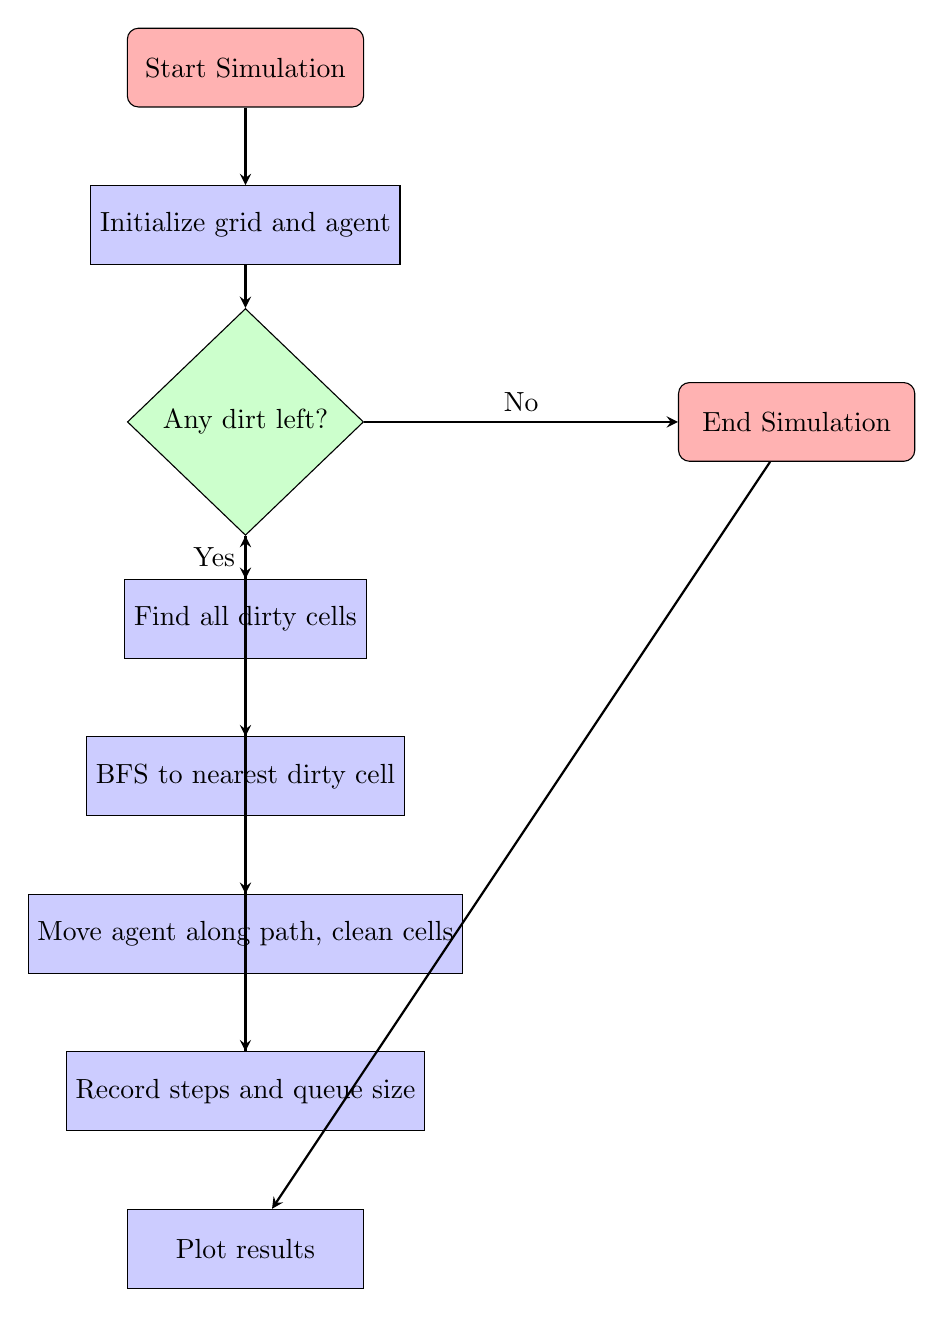
\begin{tikzpicture}[node distance=2cm]
    \node (start) [startstop] {Start Simulation};
    \node (init) [process, below of=start] {Initialize grid and agent};
    \node (dirt) [decision, below of=init, yshift=-0.5cm] {Any dirt left?};
    \node (find) [process, below of=dirt, yshift=-0.5cm] {Find all dirty cells};
    \node (bfs) [process, below of=find] {BFS to nearest dirty cell};
    \node (move) [process, below of=bfs] {Move agent along path, clean cells};
    \node (collect) [process, below of=move] {Record steps and queue size};
    \node (plot) [process, below of=collect] {Plot results};
    \node (end) [startstop, right of=dirt, xshift=5cm] {End Simulation};

    \draw [arrow] (start) -- (init);
    \draw [arrow] (init) -- (dirt);
    \draw [arrow] (dirt) -- node[anchor=east] {Yes} (find);
    \draw [arrow] (find) -- (bfs);
    \draw [arrow] (bfs) -- (move);
    \draw [arrow] (move) -- (collect);
    \draw [arrow] (collect) -- (dirt);
    \draw [arrow] (dirt) -- node[anchor=south] {No} (end);
    \draw [arrow] (end) -- (plot);
\end{tikzpicture}
\end{center}

\end{document}